% s/[0.5ex]//g to squeeze the space
%
\begin{figure*}
  \begin{center}
    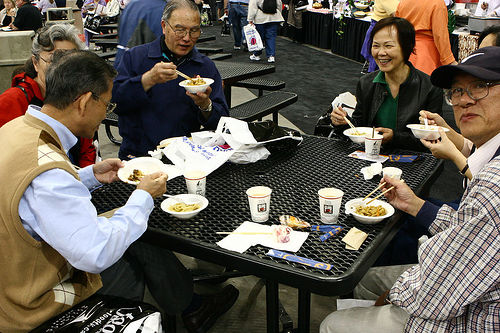
\includegraphics[width=0.4\textwidth]{chapters/ConLL/10459869.jpg}
  \end{center}
  \vspace{1em}
  \begin{subfigure}[t]{0.5\textwidth}
    \textbf{En:} A group of people are eating noodles.\\[0.5ex]
    \textbf{De:} Eine Gruppe von Leuten isst Nudeln.\\[0.5ex]
    \textbf{Fr:} Un groupe de gens mangent des nouilles.\\[0.5ex]
    \textbf{Cs:} Skupina lidí jedí nudle.\\
    \vspace{2em}
    \caption{A translation tuple}
  \end{subfigure}
  \begin{subfigure}[t]{0.5\textwidth}
    \textbf{En:} Several asian people eating around a table.\\[0.5ex]
    \textbf{De:} Drei Männer und zwei Frauen südostasiatischen Aussehens sitzen, aus Schälchen essend, an einem schwarzen, Tisch, auf dem sich u.a. auch Pappbecher und eine Tasche befinden, im Hintergrund sind weitere Personen und Tische.\footnotemark\\
    %\textbf{De:} 3 Männer und 3 Frauen essen zusammen an einem Tisch.
    \caption{A comparable pair}
  \end{subfigure}
  \caption{An example taken from the {\it Translation} and {\it Comparable} portions of the Multi30K dataset. The translation portion (a) contains professional translations of the English captions into German, French, and Czech. The comparable portion (b) consists of five independently crowdsourced English and German descriptions, given only the image. Note that the sentences in (b) convey different information from the English--German translation pair in (a).}\label{fig:data:example}
\end{figure*}
